\lecture{19}{23. April 2025}{Processing of Metals: Heat Treatment}

\section{Thermal processing of metals}

\subsection{Annealing processes}
\textit{Annealing} is the name for a form of heat treatment where a material is exposed to an elevated temperature for an extended time period and then slowly cooled. Typically this is carried out to:
\begin{itemize}
  \item Relieve stresses
  \item Increase softness, ductility and toughness
  \item Produce a specific microstructure
\end{itemize}

Any annealing process consists of three stages:
\begin{enumerate}
  \item Heating to the desired temperature
  \item Holding or ``soaking'' at that temperature
  \item Cooling, usually to room temperature 
\end{enumerate}
Time is an important parameter in these processes. During heating and cooling, temperature gradients exist between the outside and interior portions of the piece; their magnitude depend on the size and geometry of the piece. If the rate of temperature change is too great, temperature gradients and internal stresses may be induced that may lead to warping or cracking.

\subsubsection{Process annealing}
\textit{Process annealing} is a heat treatment that is used to negate the effects of cold work (i.e., to soften and increase the ductility of a strain-hardened metal). Typically a fine grained microstructure is desired, and therefore the heat treatment is terminated before appreaciable grain growth has occurred. 

\subsubsection{Stress relief}
Internal stresses may develop in pieces in response to things such as plastic deformation, nonuniform cooling or other things like that. Distortion and warpage may result if the internal stresses are not removed. They may be eliminated by a \textit{stress relief annealing} heat treatment. The annealing temperature is typically relatively low such that the effects resulting from cold working and other heat treatments are not affected.

\subsubsection{Annealing of ferrous alloys}
Many different annealing procedures are employed to enhance the properties of steel alloys.

\paragraph{Normalizing} Steels that have been plastically deformed by, e.g., a roller consists of grains of pearlite (and most likely a proeutectoid phase), which are irregularly shaped and relatively large and vary substantially in size. An annealing heat treatment called \textit{normalizing} is used to refine the grains (i.e., decrease average grain size) and produce a tougher more uniform steel. Normalizing is accomplished by heating at least \qty{55}{\celsius} above the upper critical temperature (i.e. above the hypo-/hyper-eutectoid temperature). After sufficient time has been allowed for the alloy to completely transform to austenite -- a procedure called \textit{austenizing} -- the treatment is terminated by cooling in air. 

\paragraph{Full anneal} A heat treatment known as \textit{full annealing} is often used in low- and medium-carbon steels that will be machined or will experience extensive plastic deformation during a forming operation. In general, the alloy is treated by heating to a temperature of about \qty{50}{\celsius} above the upper critical line to form austenite or austenite and $\mathrm{Fe}_3 \mathrm{C}$-phases. The alloy is then furnace cooled -- that is, the heat-treating furnace is turned off, and both furnace and steel cool to room temperature at the same rate, which takes several hours. This gives a relatively soft and ductile material with large pearlite grains.

\paragraph{Spheroidizing}
Medium- and high-carbon steels having a microstructure containing even coarse pearlite may still be too hard to machine or plastically deform conveniently. Spheroidized steels have a maximum softness and ductility and are easily machined or deformed. The \textit{spheroidizing} heat treatment, during which there is a coalescence of the $\mathrm{Fe}_3 \mathrm{C}$ to form the spheroid particles, can take place by several methods, as follows:
\begin{itemize}
  \item Heating the alloy at a temperature just below the eutectoid in the $\alpha + \mathrm{Fe}_3 \mathrm{C}$ region of the phase diagram. If the precursor microstructure contains pearlite, spheroidizing times will typically range between 15 and \qty{25}{h}.
  \item Heating to a temperature just above the eutectoid temperature and then either cooling very slowly in the furnace or holding at a temperature just below the eutectoid temperature.
  \item Heating and cooling alternately within about $\pm \qty{50}{\celsius}$ of the hypo-/hyper-eutectoid temperature.
\end{itemize}
To some degree, the rate at which spheroidite forms depends on prior microstructure.
For example, it is slowest for pearlite, and the finer the pearlite, the more rapid the
rate. Also, prior cold work increases the spheroidizing reaction rate.


\subsection{Heat treatment of steels}
Conventional heat treatment procedures for producing martensitic steels typically involve
continuous and rapid cooling of an austenitized specimen in some type of quenching
medium, such as water, oil, or air. The optimum properties of a steel that has been
quenched and then tempered can be realized only if, during the quenching heat treatment, the specimen has been converted to a high content of martensite; the formation of any
pearlite and/or bainite will result in other than the best combination of mechanical
characteristics.

\subsubsection{Hardenability}
The influence of alloy composition on the ability of a steel alloy to transform to martensite for a particular quenching treatment is related to a parameter called \textit{hardenability}. For every steel alloy, there is a specific relationship between the mechanical properties and the cooling rate. Hardenability is a term used to describe the ability of an alloyr to be hardened by the formation of martensite as a result of a given heat treatment. Hardenability is not ``hardness''. 

\paragraph{Jominy end-quench test} One standard procedure used to determine hardenability is the \textit{Jominy end-quench test}. Except for alloy composition, all factors that may influence the depth to which a piece hardens (i.e., specimen size and shape and quenching treatment) are maintained constant. A cylindrical specimen \qty{25,4}{mm} in diameter and \qty{100}{mm} long is austenized at a prescribed temperature for a prescribed time. After removal from the furnace, it is quickly mounted in the test fixture. The lower end is quenched by a jet of water of specified flow rate and temperature. Thus, the cooling rate is at a maximum here and diminishes from this end and through the test-specimen. After the specimen has cooled to room-temperature shallow flats \qty{0,4}{mm} deep are cut into the specimen where a Rockwell hardness test is made. From this a hardenability curve depicting hardness versus distance from quenched end can be made. 

Possibly write more here idk :)


\subsection{Precipitation hardening}
One can also elect to introduce particles of a seperate phase within the original phase matrix. This is called \textit{precipitation hardening}. 

\paragraph{Heat treatments} Two requisite features must be displayed by a phase diagram of an alloy system for precipitation hardening: an appreciable maximum solubility of one component in the other, on the order of several percent; and a solubility limit that rapidly decreases in concentration of the major component with temperature reduction. 

\paragraph{Solution heat treating} Precipitation hardening is accomplished by two different heat treatments. The first is a \textit{solution heat treatment} in which all solute atoms are dissolved to form a single phase solid solution. This procedure is followed by rapid cooling to quenching to a temperature which for many alloys is room temperature, to the extent that any diffusion and accompanying formation of any of the $\beta$ phase are prevented. This a nonequilibrium situation exists.

\paragraph{Precipitation heat treating} For the second or \textit{precipitation heat treatment} the supersaturated $\alpha$ solid solution is ordinarily heated to an intermediate temperature within the $\alpha + \beta$ phase region. The $\beta$ precipitate begins to form as finely dispersed particles of composition $C_{\beta}$ which is sometimes called \textit{aging}. After the appropriate aging time the alloy is cooled to room temperature: normally, the cooling rate here is not important. For some alloys, aging occurs spontaneously at room temperature over extended time periods. 

\subsection{Mechanism of hardening}
Precipitation hardening is commonly employed with high-strength aluminum alloys. Perhaps the most commonly studied aluminum alloy is with copper as shown on \textbf{\autoref{fig:e19_5}}.
\begin{figure} [ht]
  \centering
  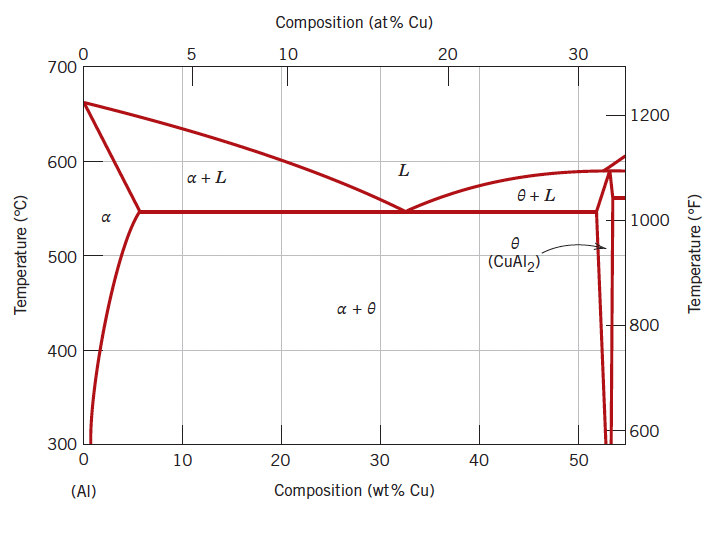
\includegraphics[width=0.5\linewidth]{./figures/e19_5.png}
  \caption{Aluminum-rich side of aluminum-copper phase diagram}
  \label{fig:e19_5}
\end{figure}

The $\alpha$-phase is a substitutional solid solution of copper in aluminum, whereas the intermetallic compund $\mathrm{CuAl}_2$ is designated the $\theta$ phase. For an aluminum-copper alloy of, say, composition \qty{96}{wt\% Al}--\qty{4}{wt\% Cu}, in the development of this equilibrium $\theta$ phase during the precipitation heat treatment, several transition phases are first formed in a specific sequence. During the initial hardening stage (at short times), copper atoms cluster together in very small thin discs that are only one or two atoms thick and approximately \qty{25}{atoms} in diameter; these form at countless positions within the $\alpha$ phase. The clusters, also called \textit{zones}, are so small that they are not really regarded as distinct precipitate particles. However, with time and the subsequent diffusion of copper atoms, zones become particles as they increase in size. These precipitate particles then pass through two transition phases (denoted $\theta''$ and $\theta'$), before the formation of the equilibrium $\theta$ phase. Maximum strength conincides with the formation of the $\theta''$ phase, which may be preserved upon cooling to room temperature. The strengthening process is accelerated as the temperature is increased. 
